%%%%%%%%%%%%%%%%%%%%%%%%%%%%%%%%%%%%%%%%%%%%%%%%%%%%%%%%%%%%%%%%%%%%
\newpage
\phantomsection
\addcontentsline{toc}{section}{A. Presentations}
\label{sec:sourcecode}
{\Huge \bf \noindent B. PRESENTATIONS}

\newpage
\phantomsection
\addcontentsline{toc}{subsection}{A.1 ServalDHT - Secure DHT based Service Resolution Service}
\label{sec:servaldhtpres}
{\huge \bf \noindent A.1 ServalDHT - Secure DHT\\[0.2cm] based Service Resolution Service}
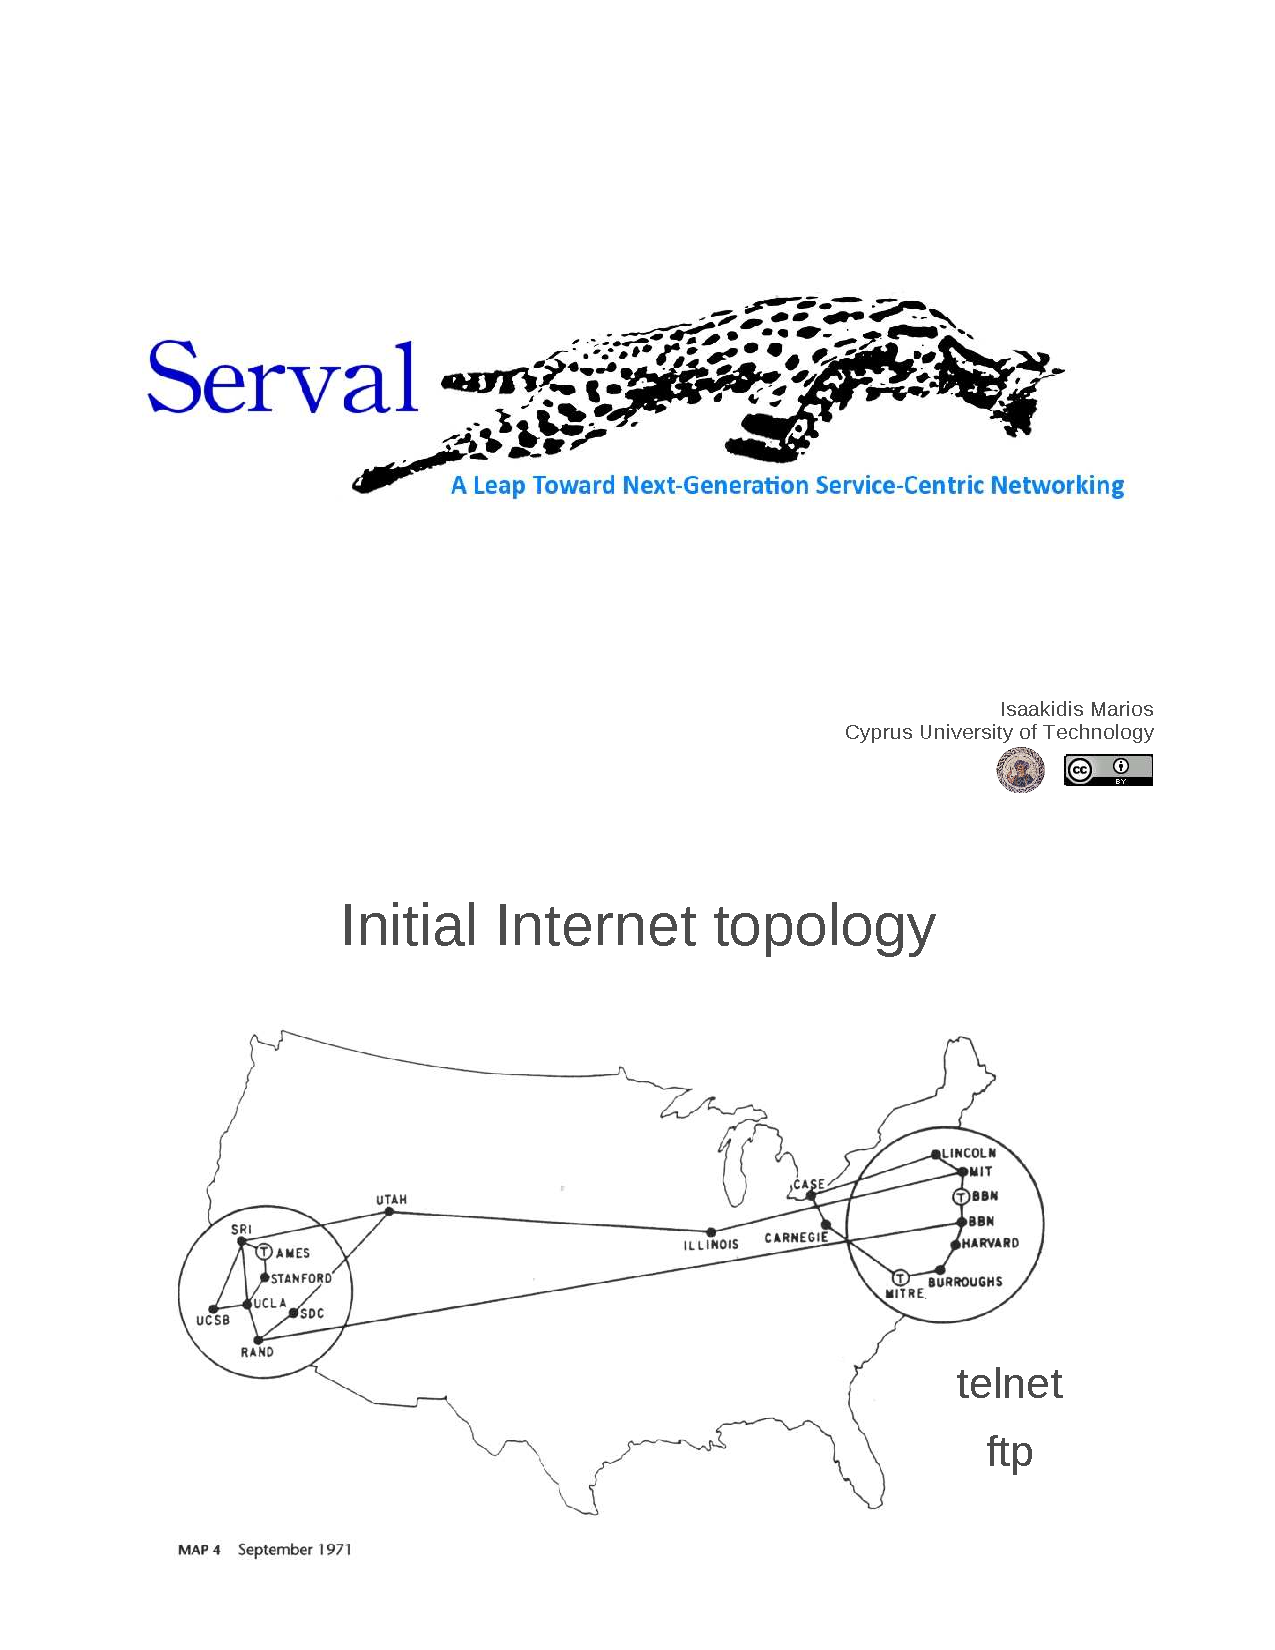
\includepdf[pages={-}]{ServalDHT-Pres2.pdf}


%%%%%%%%%%%%%%%%%%%%%%%%%%%%%%%%%%%%%%%%%%%%%%%%%%%%%%%%%%%%%%%%%%%%
\newpage
\phantomsection
\addcontentsline{toc}{section}{B. Source Code}
\label{sec:sourcecode}
{\Huge \bf \noindent B. SOURCE CODE}


%%%%%%%%%%%%%%%%%%%%%%%%%%%%%%%%%%%%%%%%%%%%%%%%%%%%%%%%%%%%%%%%%%%%
\newpage
\phantomsection
\addcontentsline{toc}{subsection}{B.1 nginx Serval integration}
\label{sec:nginxport}
{\huge \bf \noindent B.1 nginx Serval integration}\\[0.5cm]
\textbf{File:} ports/nginx/nginx-1.2.9-integrated-serval.patch\\
\textbf{Description:} Integrate Serval patch nginx version 1.2.9 in the build procedure.\\
\textbf{Instructions: }
\begin{enumerate} \itemsep1pt \parskip0pt 
\parsep0pt
	\item Apply the patch using git to nginx\_1.2.9\_serval\_fqdn branch.
	\item Copy libraries from serval/include to a path included in the search path of your compiler (normally that should be /usr/local/include/)
	\item Configure nginx with serval (ports/nginx/configure --with-serval)
	\item Make sure configure script found netinet/serval.h library and can build AF\_SERVAL
	\item If everything is fine, you should be able to see "+ using serval active sockets" in the configuration summary
	\item Compile with make and then execute make install
	\item Edit nginx configuration file (by default /usr/local/nginx/conf/nginx.conf) and uncomment the virtual host configured for the serval architecture
	\item Restart nginx and now you can accept both AF\_INET and AF\_SERVAL requests
	\item nginx Service ID is 8\\[0.5cm]
\end{enumerate}
\lstinputlisting[language=diff]{source_code/nginx-serval-build-patch.diff}

%%%%%%%%%%%%%%%%%%%%%%%%%%%%%%%%%%%%%%%%%%%%%%%%%%%%%%%%%%%%%%%%%%%%
\newpage
\phantomsection
\addcontentsline{toc}{subsection}{B.2 Wireshark Lua Serval Dissector}
{\huge \bf \noindent B.2 Wireshark Lua Serval Dissector}\\[0.5cm]
\textbf{File:} serval/src/serval\_wireshark\_dissector.lua\\
\textbf{Description:} Wireshark dissector for the Serval protocol (IPPROTO\_SERVAL 144).\\
\textbf{Instructions: }
\begin{enumerate} \itemsep1pt \parskip0pt 
\parsep0pt
	\item Make sure Lua is enabled in wireshark's global configuration (\href{http://wiki.wireshark.org/Lua}{Wireshark wiki})
	\item Copy serval/src/serval\_wireshark\_dissector.lua into a plugin directory (default is $\sim$/.wireshark/plugin)\\[0.5cm]
\end{enumerate}
\lstinputlisting[language=lua]{source_code/serval_wireshark_dissector.lua}

%%%%%%%%%%%%%%%%%%%%%%%%%%%%%%%%%%%%%%%%%%%%%%%%%%%%%%%%%%%%%%%%%%%%
\newpage
\phantomsection
\addcontentsline{toc}{subsection}{B.3 Initialize Serval test node Script}
{\huge \bf \noindent B.3 Initialize Serval test node Script}\\[0.5cm]
\textbf{File:} serval/src/init\_servtest.sh\\
\textbf{Description:} Initialize a Serval testing node.\\
\textbf{Instructions: }
\begin{enumerate} \itemsep1pt \parskip0pt 
\parsep0pt
	\item You might want to set the executable bit (chmod +x init\_servtest.sh)
	\item Execute the script with superuser privileges
	\item View help with \texttt{-}h\\[0.5cm]
\end{enumerate}
\lstinputlisting[style=BashColor]{source_code/init_servtest.sh}

%%%%%%%%%%%%%%%%%%%%%%%%%%%%%%%%%%%%%%%%%%%%%%%%%%%%%%%%%%%%%%%%%%%%
\newpage
\phantomsection
\addcontentsline{toc}{subsection}{B.4 HTTP Client}
{\huge \bf \noindent B.4 HTTP Client}\\[0.5cm]
\textbf{File:} serval/src/test/http\_client.c\\
\textbf{Description:} HTTP client that works with both AF\_SERVAL and AF\_INET families.\\
\textbf{Instructions: } Print usage with \texttt{-}h or \texttt{{-}{-}}help\\[0.5cm]
\lstinputlisting[style=CColor]{source_code/http_client.c}

%%%%%%%%%%%%%%%%%%%%%%%%%%%%%%%%%%%%%%%%%%%%%%%%%%%%%%%%%%%%%%%%%%%%
\newpage
\phantomsection
\addcontentsline{toc}{subsection}{B.5 libmicrohttpd Serval port}
{\huge \bf \noindent B.5 libmicrohttpd Serval port}\\[0.5cm]
\textbf{File:} ports/libmicrohttpd-0.9.36/libmicrohttpd\_serval.patch\\
\textbf{Description:} Patch libmicrohttpd version 0.9.36 to use Serval active sockets. Libmicrohttpd is a small C library that can be included in other C applications and provide HTTP server functionality.\\
\url{https://www.gnu.org/software/libmicrohttpd/}\\
\textbf{Instructions: }
\begin{enumerate} \itemsep1pt \parskip0pt 
\parsep0pt
	\item Add\\[0.5cm]
\end{enumerate}
\lstinputlisting[language=diff]{source_code/libmicrohttpd_serval.patch}